%! Licence = CC BY-NC-SA 4.0

%! Author = gianfluetsch
%! Date = 19. Jan 2022
%! Project = pfsec_summary

\section{Identity and Access Management (IAM)}

\subsection{Towards an IAM}

\subsubsection{Identification}
\begin{center}
    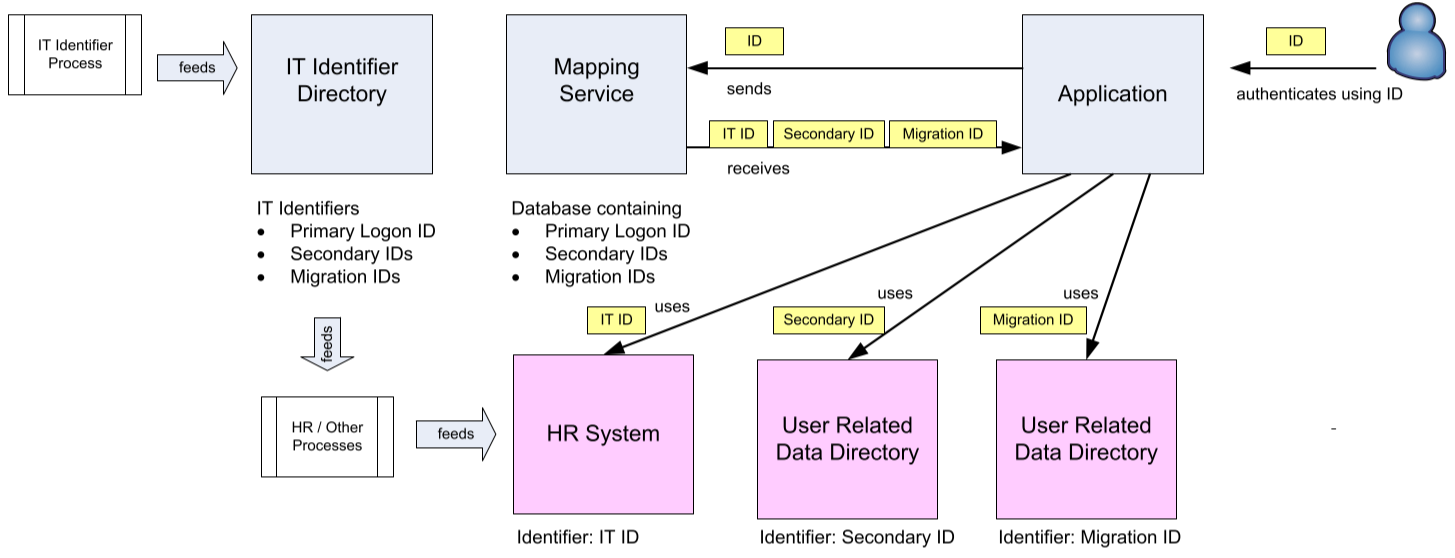
\includegraphics[width=.9\linewidth]{05-iam/identification}
    \vspace{-8pt}
\end{center}

\subsubsection{Authentication}
\begin{center}
    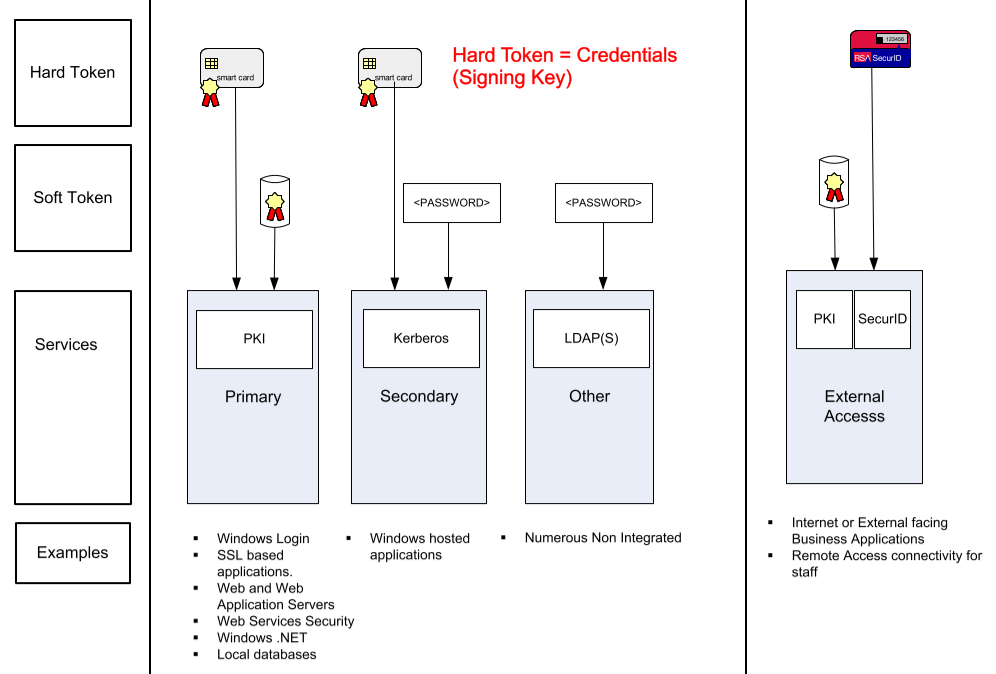
\includegraphics[width=.9\linewidth]{05-iam/authentication}
    \vspace{-8pt}
\end{center}

\subsubsection{Principle Propagation}
\begin{minipage}{0.5\linewidth}
    In a multi-tiered architecture, principal propagation is important. Whenever a principal (user or another application) is authenticated, a \textit{security context} is created. That context may be system, environment or even mechanism dependent. \textit{But that security context should contain reliable trustworthy identity data that corresponds to an authenticated principal}.\\

    During propagation, \textit{the security context is transferred from one trusted tier to the next trusted one}. Each server application can obtain the authenticated identification of the client principle from the security context. The use of the authenticated identity is necessary for the correct creation of accountability data and the correct application of authorization policies.\\
\end{minipage}
\begin{minipage}{0.45\linewidth}
    \begin{center}
        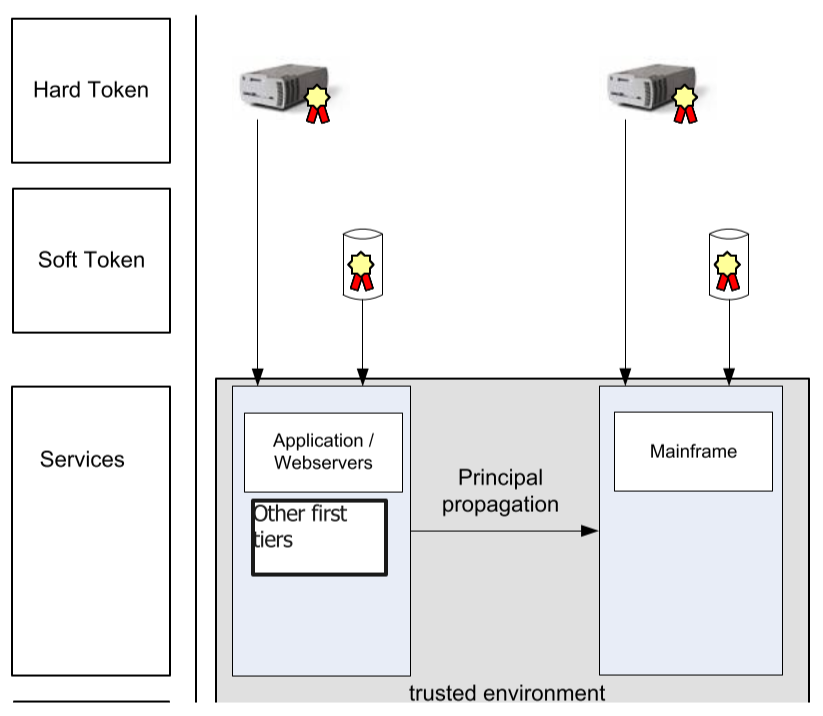
\includegraphics[width=.9\linewidth]{05-iam/principle_propagation}
        \vspace{-8pt}
    \end{center}
\end{minipage}

\textcolor{red}{Deshalb wird in grossen Umgebungen oft mit \textbf{PKI (Public-Key-Infrastructure)} gearbeitet.}

\begin{center}
    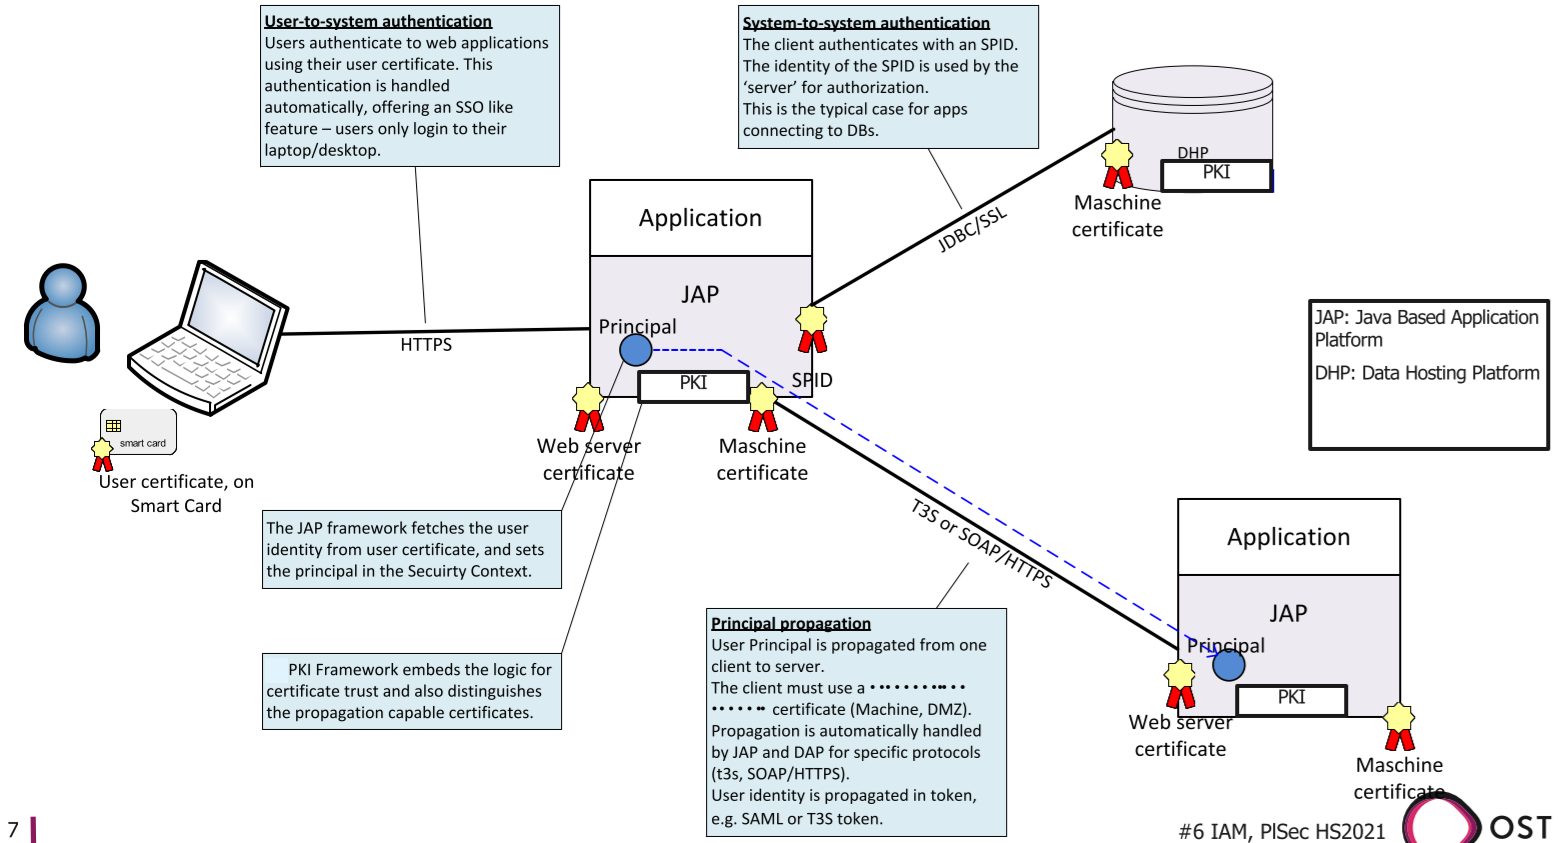
\includegraphics[width=.9\linewidth]{05-iam/pki}
    \vspace{-8pt}
\end{center}

\subsubsection{Access Control}\label{subsubsec:access-control}
\begin{center}
    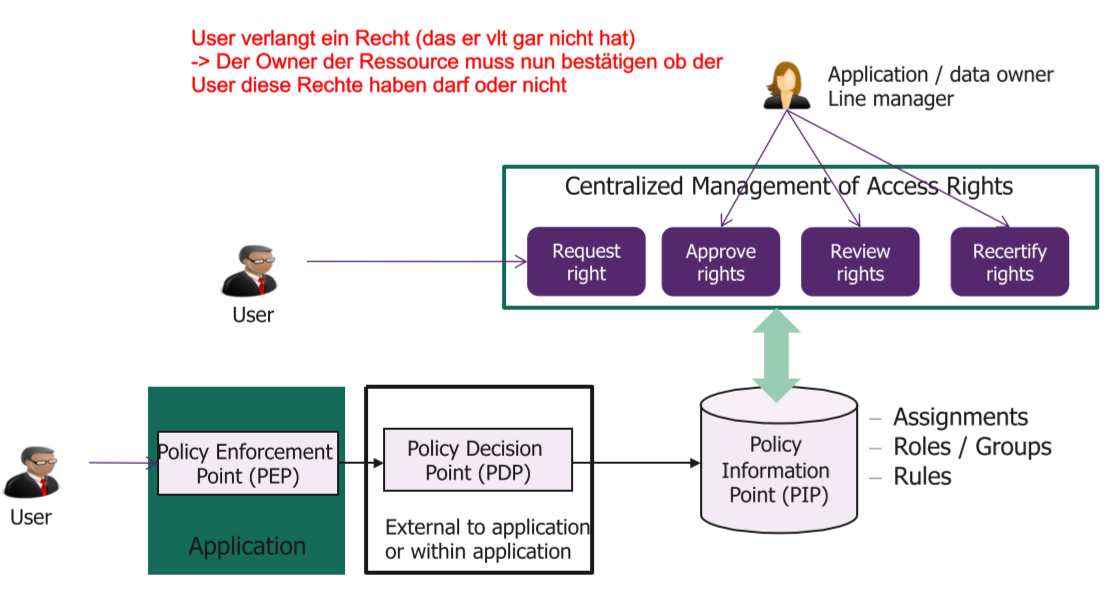
\includegraphics[width=.7\linewidth]{05-iam/access_control}
    \vspace{-8pt}
\end{center}

\newpage

\paragraph{Options for Integration with centralized access control}
\begin{center}
    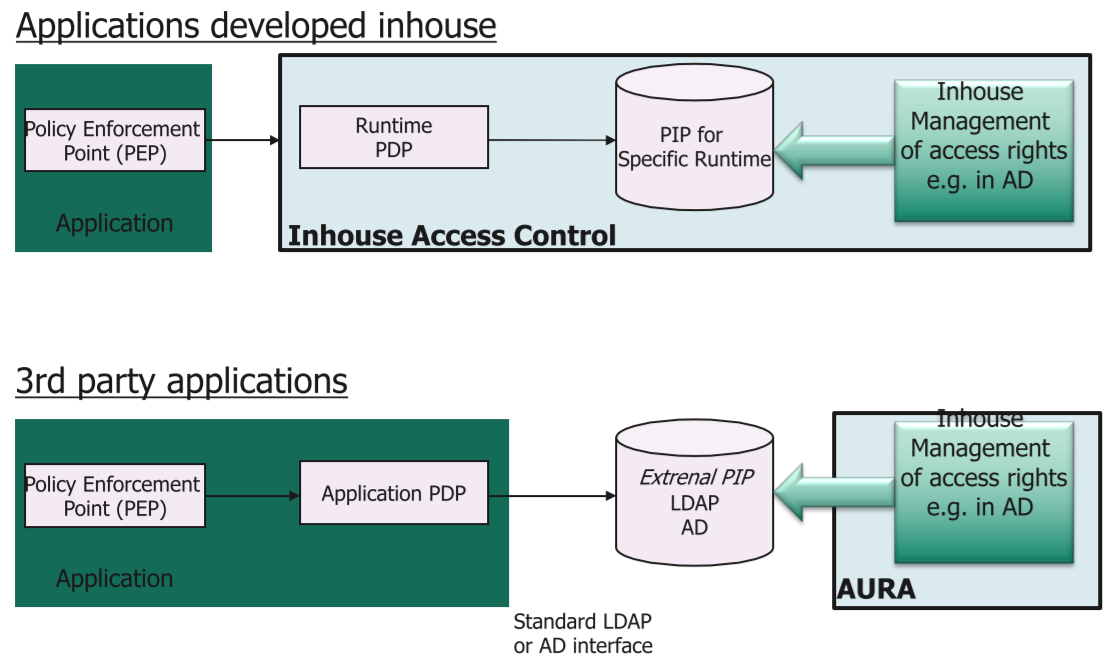
\includegraphics[width=.7\linewidth]{05-iam/access_control2}
    \vspace{-8pt}
\end{center}

\subsubsection{Typical Solutions}
\begin{table}[h]
    \centering
    \begin{tabular}{p{2cm} | p{4cm} | p{5cm} | p{4cm}}
        \bfseries{Solutions} & \bfseries{Description} & \bfseries{Use Cases} & \bfseries{Level, PDP, PIP}\\ \hline
        Active Directory & User is known in AD, AD objects have ACLs (users, groups), AD makes decision & Windows based applications (in future with AD bridge eventually Unix/Linux based applications) & 
        \begin{itemize}
            \item Level: Functional
            \item PDP: AD
            \item PIP: AD
            \item Example: AD
        \end{itemize}\\
        LDAP/DB call & Application calls an LDAP or DB to validate a group membership, depending on the result application decides & Any application using the access control LDAP, AD or appl. individual LDAP/DB to retrieve group memberships or other attributes &
        \begin{itemize}
            \item Level: Functional
            \item PDP: Application
            \item PIP: LDAP, DB
            \item Example: AD
        \end{itemize}\\
        External Policy Decision Point (PDP) & Application externalizes decision to a policy decision point & Self developed applications using AURA ARQs, COTS supporting XACML or applications with individual AbAC or PbAC engine &
        \begin{itemize}
            \item Level: Functional and Data
            \item PDP: external engine
            \item PIP: LDAP, DB
        \end{itemize}\\
        OS-Security & User is known to the OS, access rights on processes or files are defined on OS-Level ACLs, OS makes decision & Access control for technical user (SPIDs). Access control for system level operation that cannott be proxified by sys mgmt tools &
        \begin{itemize}
            \item Level: Functional Level
            \item PDP: OS
            \item PIP: OS
        \end{itemize}
    \end{tabular}
\end{table}

\subsubsection{Role Model and Provisioning}
\begin{center}
    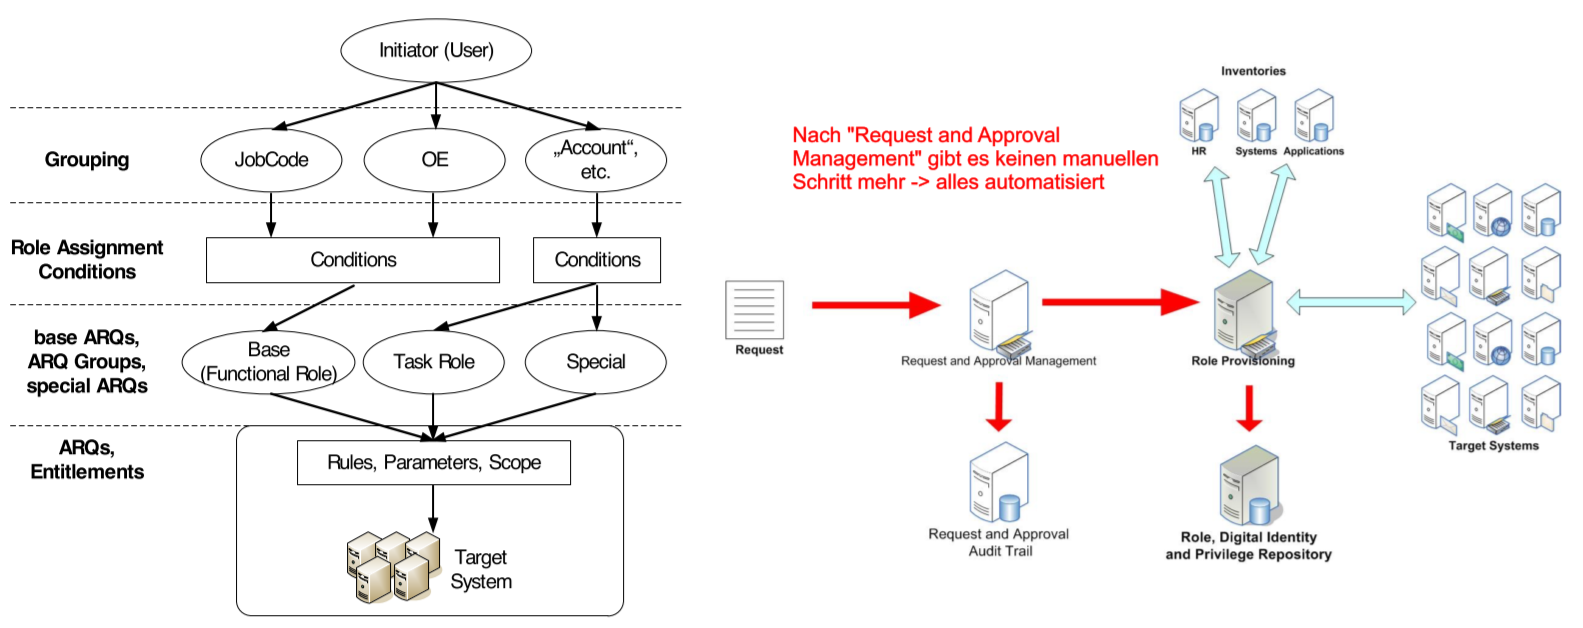
\includegraphics[width=1.0\linewidth]{05-iam/role_model}
    \vspace{-8pt}
\end{center}

\subsection{IAM Architectures}

\subsubsection{Hybrid Cloud-On-premise IAM}
\begin{center}
    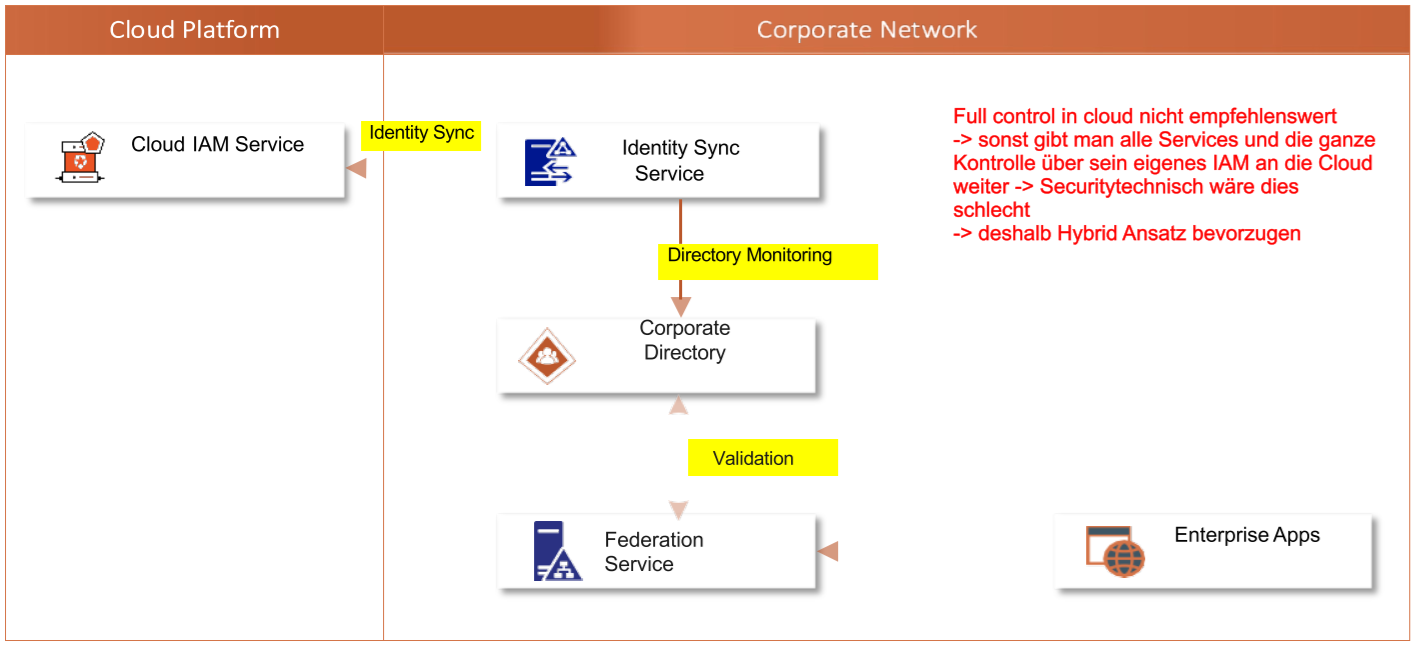
\includegraphics[width=.9\linewidth]{05-iam/hybrid}
    \vspace{-8pt}
\end{center}

\begin{table}[h]
    \centering
    \begin{tabular}{p{4cm} | p{12cm}}
        \bfseries{Component} & \bfseries{Description}\\ \hline
        On-Premise (Corporate Directory) & Directory service that enables authentication to access enterprise resources (e.g., Active Directory). Typically contains directory objects (accounts) that represent a human (user account) or non-human identity (service account).\\ \hline
        On-Premise Federation Service & Identity service that implements common access management capabilities (authentication and authorization) for enterprise applications. Typically supports identity standards like SAML or OpenID Connect to enable access to internal or external resources.\\ \hline
        Identity Sync Service & Infrastructure service that monitors directory objects in the enterprise directory for changes and synchronizes changes to a mapped cloud directory object. Sync direction can be one-way or two-way but is typically implemented in an Enterprise to Cloud direction to minimize risk and complexity. Standards such as SCIM can be used for this data transfer.\\ \hline
        Cloud IAM Service & Platform service in a public cloud that implements core IAM capabilities (Authentication, Federation, Access Management) and can be leveraged to access on-premise resources as well.
    \end{tabular}
\end{table}

\paragraph{Considerations for a Hybrid IAM}
\begin{itemize}
    \item \textbf{User Provisioning}
    \begin{itemize}
        \item User objects can be configured to synchronize when added to either the cloud or the on-premises environment.
        \item The best practice is to \textit{restrict user provisioning to one environment and sync account and profile data to the other environment} (typically from enterprise to the cloud).\\
    \end{itemize}
    \item \textbf{Profile Data}
    \begin{itemize}
        \item Manually maintaining identities in more than one environment can add unnecessary complexity and risk to your security posture.
        \item Cloud identity objects may not need the entire set of user profile data available for an on-premises user.
        \item The IAM practitioner should take care (e.g., understand the business requirements for authentication) when deciding how much user profile data should be stored on a cloud user object. A principle of \textit{''least privilege''} should be applied to avoid data spillage.\\
    \end{itemize}
    \item \textbf{Single Sign-On}
    \begin{itemize}
        \item Cloud IAM environments can \textit{enable SSO to on-premises applications or services}.
        \item For SSO to be successful, the user object must have been \textit{provisioned} and \textit{enabled for sign-in}.
        \item It is critical to understand the authentication scenarios available from the cloud IAM platform (e.g., pass-through authentication or federation) and ensure that there is a fit with the enterprise requirements.\\
    \end{itemize}
\end{itemize}

Normalerweise gibt es Master-Slave-Environment.

\subsubsection{OAuth 2.0}
\begin{center}
    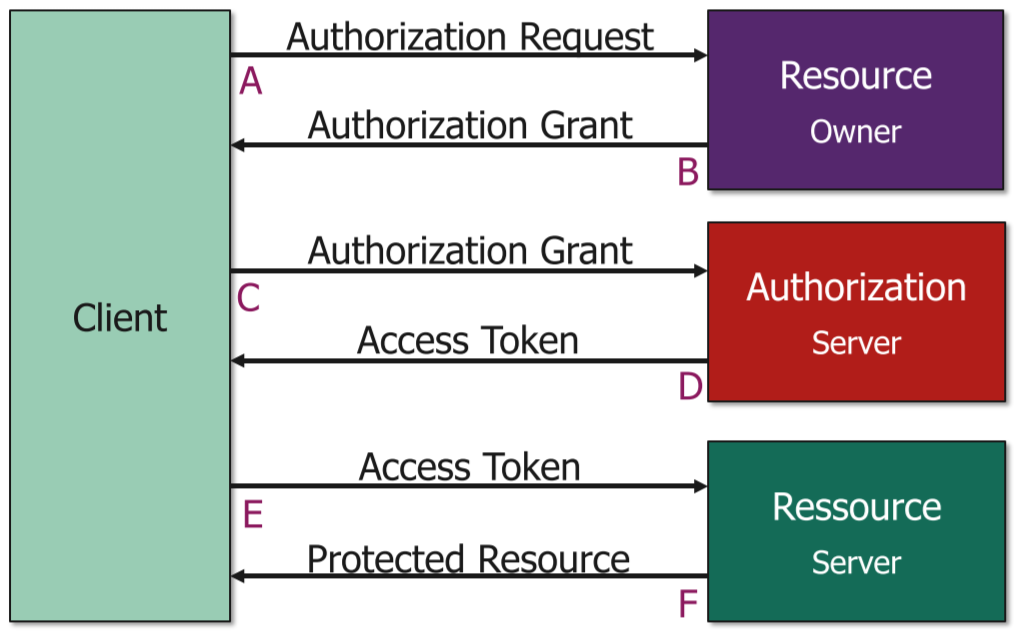
\includegraphics[width=.5\linewidth]{05-iam/oauth}
    \vspace{-8pt}
\end{center}

% TODO: üabig relevant?
